\chapter{リファクタリング}\label{ch:ref}
\section{目的}
長時間動作するプログラムのトレースログは膨大な量となるため、トレースロ
グ解析を高速化する必要がある。しかし、標準形式トレースログへの変換及び
図形データの生成に関するソースコードが複雑化しているため、高速化のため
の変更を加えることが難しい。

そこで、この問題を改善するために、関連するソースコードを対象に、複雑化
させている原因を調査する。
その後、その原因を対象するための
リファクタリング方針の決定を行なう。

\section{対象}
調査対象となったクラスは6個であり、合計行数は1590行であった。

%%      279 TraceLogVisualizerData/TraceLogGenerator.cs
%%      327 TraceLogVisualizerData/StandardFormatConverter.cs
%%      516 VisualizeShapeData/EventShapesGenerator.cs
%%      320 TraceLogData/TraceLogData.cs
%%      148 ../Base/TLVFunction.cs
%%     1590 total

\section{発見した問題点と改善方法}
クラスを調査した結果、各クラスの単一の責務を持ち、過度に結合しているク
ラスも存在しなかった。そのため、クラス設計について大きな問題はない。

しかし、多くのクラスにおいて、複雑な処理を行なうメソッドが存在しており、これが
ソースコードを複雑化さている原因である。

そこで、メソッドの整理するための共通機能のくくりだしやクラス分割をリファクタリングの目的とした。

\subsection{標準形式トレースログのパーシングにおける正規表現の多用}
標準形式トレースログのパーシングにおいて、\figref{fig:regexp}のように複
雑な正規表現を多用されていた。複雑な正規表現が用いられているため、可読
性が低く、保守も難しい。

これを改善するためは、正規表現ではなく文脈自由文法を扱えるパーサを採用
する必要がある。パーサの実現方法について、次の2つの方針を比較・検討した。

1つ目は、Yaccなどのコンパイラ・コンパイラを用いて、パーサを生成する方針
である。高速なパーサを生成でき、またコンパイラ・コンパイラの種類によっ
てはLALR文法という強力な文法を利用可能である。構文定義を更新するたびにパー
サを再生成させる必要がある。また、デバッグには、そのコンパイラ・コンパ
イラ固有の知識が要求される。

2つ目は、Parsec\cite{parsec}などに代表されるパーサ・コンビネータを実装
し、その上でパーサを記述する方針である。構文定義を更新するたびにパーサ
を再生成する必要がなく、デバッグも通常のプログラムとは同様に行なえる。
しかし、利用可能な文法がLL(k)文法なので左再帰の除去などが必要となる。ま
た、パーサ・コンビネータを実装する必要があるため実装コストが高い。

両手法で利用可能な文法のクラスは包含関係にないため、表現能力を単純に比
較することはできない。トレースログのパーシングは比較的単純であるため、
どちらを用いても問題ない。

パーサを再生成する必要がない点と、デバッグの容易さなど
から、2つめのパーサ・コンビネータを用いる方針を採用した。

\begin{figure}
\centering
\begin{lstlisting}
...
m = Regex.Match(_log, @"\[(?<time>[0-9a-zA-Z]+(\.[0-9a-zA-Z]*)?)\]");
if (m.Success)
	Time = m.Groups["time"].Value;
HasTime = m.Success;

m = Regex.Match(_log, @"^(\[[^\]]+\])?(?<object>[^\[\]\(\)\.]+(\([^\)]+\))?)(\.[^\s]+)?$");
if (m.Success)
	Object = m.Groups["object"].Value;

m = Regex.Match(_log, @"^(\[[^\]]+\])?(?<objectName>[^\[\]\(\)\.]+)(\.[^\s]+)?$");
if (m.Success)
	ObjectName = m.Groups["objectName"].Value;
HasObjectName = m.Success;

m = Regex.Match(_log, @"^(\[[^\]]+\])?(?<objectType>[^\[\]\(\)\.]+)\([^\)]+\)(\.[^\s]+)?$");
if (m.Success)
	ObjectType = m.Groups["objectType"].Value;
HasObjectType = m.Success;
...
\end{lstlisting}
\caption{正規表現を多用した例}\label{fig:regexp}
\end{figure} % $

\subsection{可視化ルールにおける暗黙的な木構造}
\begin{figure}
\centering
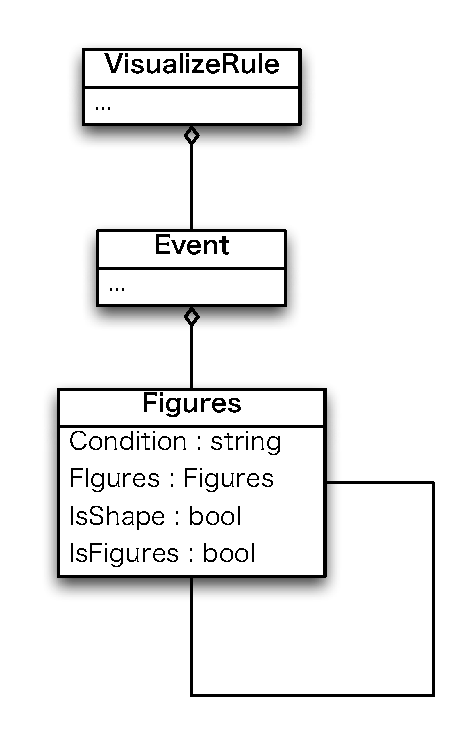
\includegraphics[width=0.3\textwidth]{current.eps}
\caption{現状の可視化ルール}\label{fig:current}
\end{figure}

\begin{figure}
\centering
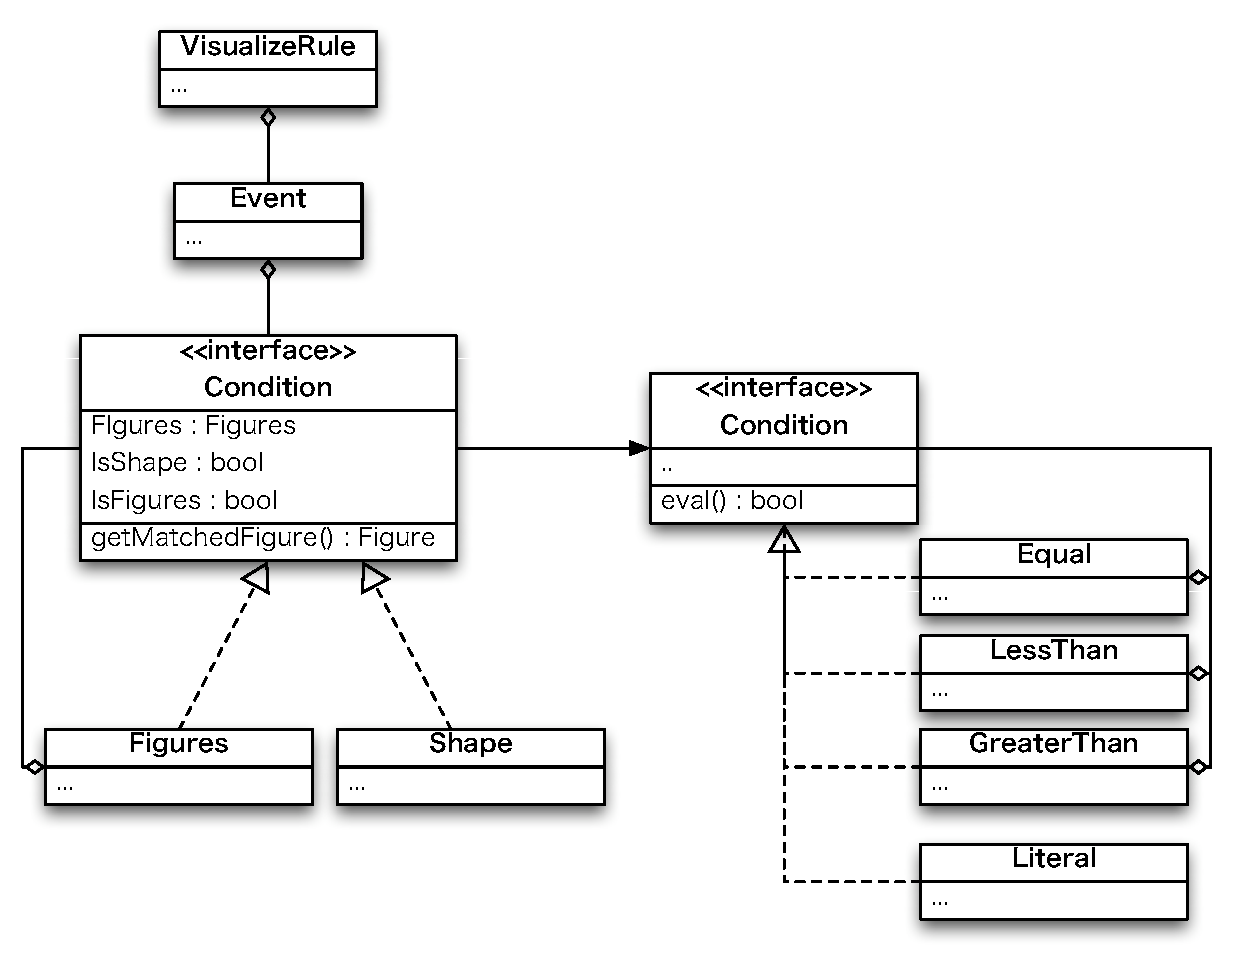
\includegraphics[width=\textwidth]{composite.eps}
\caption{Compositeパターンの適用}\label{fig:composite}
\end{figure}

\begin{figure}
\centering
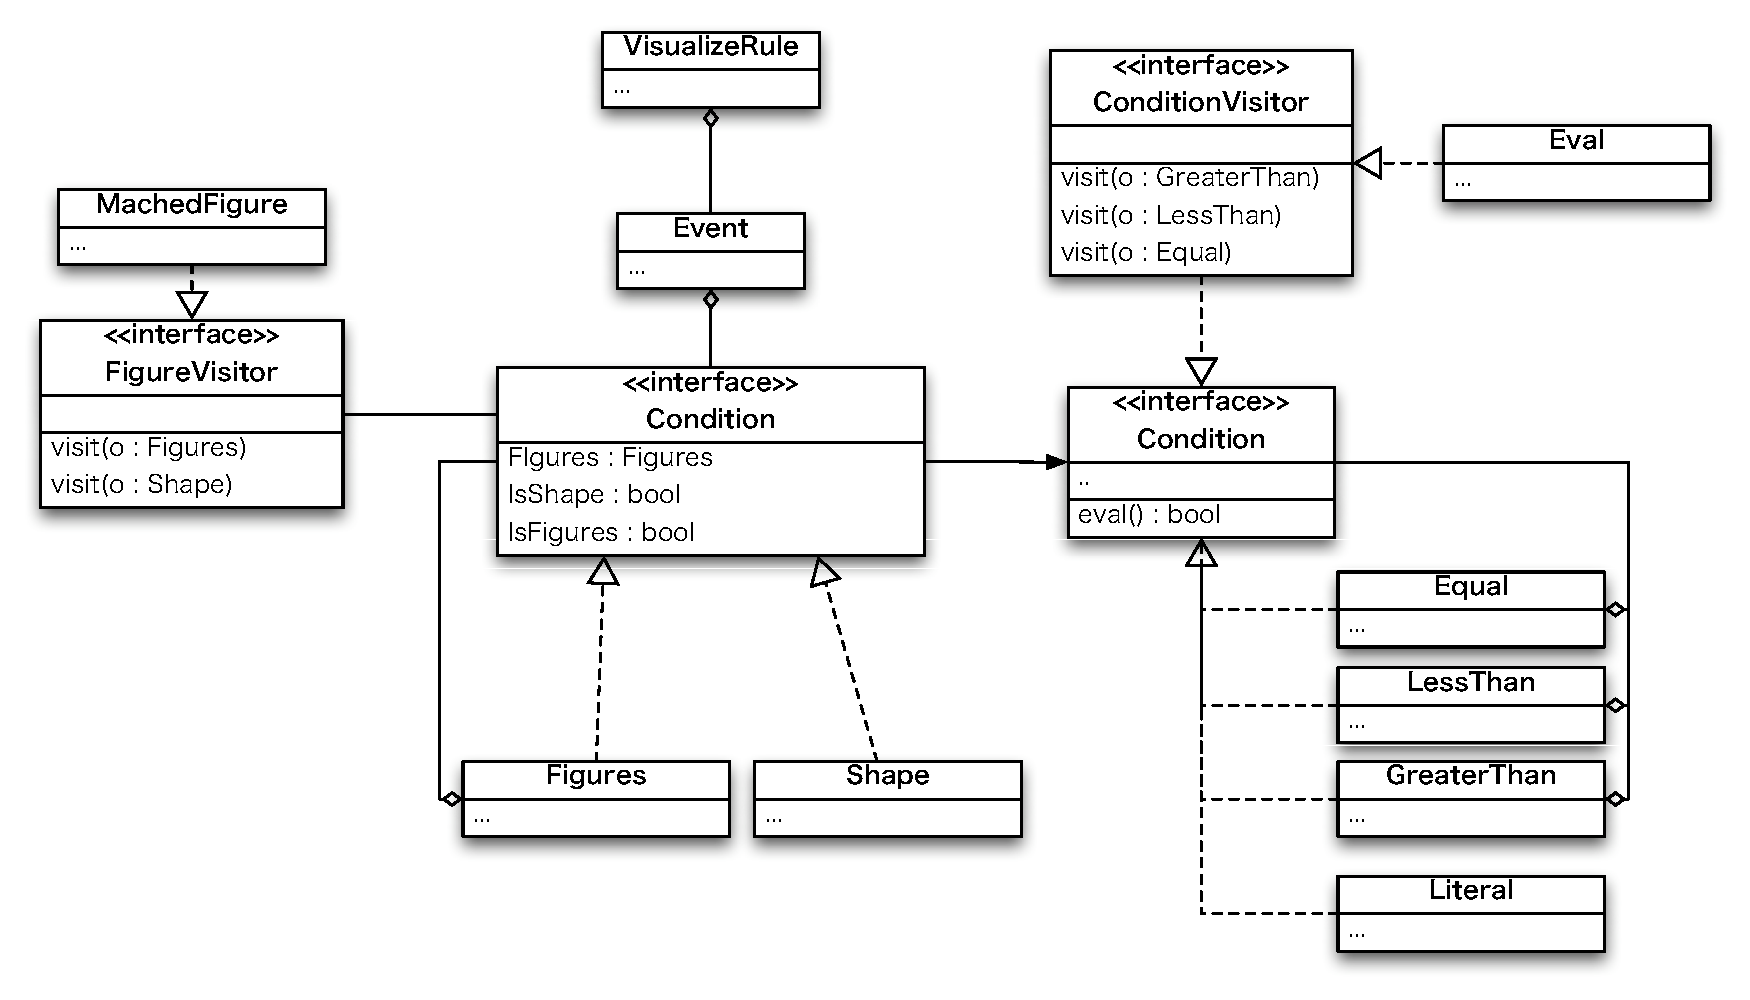
\includegraphics[width=\textwidth]{visitor.eps}
\caption{Visitorパターンの適用}\label{fig:visitor}
\end{figure}

可視化ルールは\figref{fig:current}のように、複数の\code{Figures}の集約
によって表現される。\code{Figures}にはShapeとFiguresの二種類が存在し、
Figuresは複数のShapeによって構成される。また\code{Figures}の\code{Condition}
フィールドに、その図形を用いる条件式が格納されている。条件式には、等号、
不等号、論理和、論理積などがある。

\code{Figures}クラスと\code{Condition}フィールドは木構造を持つデータであるが、木構造によって表現されていない。そのため、
木構造をトラバースするためのコードが多数の場所に存在し、
保守性と可読性が低下している。

木構造によって表現するためにCompositeパターン\cite{gof}を適用し、
\figref{fig:composite}のようにする。\code{Figures}クラスを
\code{Figure}インタフェース、枝である\code{Figures}クラス、葉である
\code{Shape}クラスに分解する。また、\code{Figures}クラスに関連した処理
を\code{Figures}クラスと\code{Shape}クラスに移動させる。同様に、
\code{Condition}フィールドを\code{Condition}インタフェースと派生クラス
に分解する。

しかし、Compositeパターンを用いると、処理を追加する際の変更範囲が大きく
なってしまう。例えば、\code{Condition}インタフェースに関する処理を追加
する場合は、\code{Equal}クラス、\code{LessThan}クラス、
\code{GreaterThan}クラス、\code{Literal}クラスを全て変更する必要がある。

そこで、\figref{fig:visitor}のようにVisitorパターンを適用し、処理を外部
のクラスへと分離する。これにより、処理の追加が容易になる。

Visitorパターンを用いた場合、構造を変更する際の修正範囲が広くなる。
しかし、可視化ルールの構造はこれまで変更が行なわれておらず、また今後も予定はない。
そのため問題ないと判断した。

